\documentclass[a4paper,10pt]{article}
\usepackage[utf8]{inputenc}
\usepackage{graphicx}
\usepackage{float}

\title{Analiza podatkov Food And Drug Administration z orodjem Bokeh}
\author{Neža Belej (63120340), Matej Dolenc (63120178)}

\begin{document}

\maketitle
\section {Bokeh}
Bokeh je interaktivna knjižnica programskega jezika Python. Omogoča elegantno in interaktivno vizualizacijo nad veliko množico podatkov.
Arhitektura Bokeha sestoji iz dveh delov: izdelava grafov z programskem jeziku Python in pa izris v brskalniku s knjižnico BokehJS. Grafi v Pythonu se pretvorijo v JSON format, saj to zahteva BokehJS. Takšen dizajn je zelo fleksibilen, saj omogoča, da delo tudi z drugimi programskimi jeziki (R, Scala, Lua,... ) lahko privede do enakih Bokeh grafov v brskalniku. \\
Če želimo sinhronizacijo Bokeh grafov in interaktivne vizualizacije v brskalniku, moramo uporabiti tudi strežnik Bokeh. Tako imamo omogočeno avtomatično posodabljanje uporabniškega vmesnika v brskalniku glede na naše klike in vnose.

\subsection{Težave}
Med spoznavanjem orodja Bokeh smo opazili, da ima orodje še kar nekaj hroščev. V okviru izdelave smo velikokrat naleteli na repozitorij na Githubu, kjer je trenutno kar 764 odprtih nalog ("issues"): \\ https://github.com/bokeh/bokeh/issues . \\Orodje je preprosto za uporabo, ima dobro dokumentacijo, vendar ima še veliko lukenj. Primer: \\
Ob prikazu grafa najpogostejših reakcij smo želeli na interaktiven način izvesti prikaz reakcij v različnih časovnih obdobjih.
Zato smo najprej želeli uporabiti element DatePicker, kjer bi lahko izbrali začetni in končni datum. Opazili smo, da ima element v trenutni fazi zelo slab izgled \\  (issue: https://github.com/bokeh/bokeh/issues/4503). Zato smo poizkusili z uporabo elementa DateRangeSlider, ki naj bi imel na različnih straneh drsnika začetni in končni datum. Element se ni prikazal \\ (issue: https://github.com/bokeh/bokeh/issues/2268 ). Zato smo bili primorani uporabiti dva navadna drsnika, enega za začetno, drugo za končno leto. 

\section{OpenFDA}
OpenFDA (Food and Drug Administration) nam na svojih straneh omogoča dostop do 100 GB velike množice podatkov, kjer lahko poizvedujemo o medicinskih poročilih o zdravilih in hrani; na primer stranski učinki zdravil ali odpoklic prehrambenih produktov. OpenFDA je namenjena predvsem za poizvedbe preko njihovega zmogljivega API-ja, ki ima v ozadju implementiran učinkovit Elastic Search. Ta nam omogoča hitro in preprosto poizvedovanje po podatkih. \\
Podatki, namenjeni prenosu, so razbiti na veliko število datotek v JSON formatu. Če želimo prenesti podatke, moramo paziti, da ob vsaki posodobitvi podatkov znova prenesemo celotno zbirko podatkov. Podatki so v dokumentni, nenormalizirani obliki, kar omogoča hitro iskanje.
\section{Navodila za izvajanje}
Za zagon projekta je potrebno imeti nameščeno orodje Anaconda. Nato iz konzole Bash ali pa Windows-ovega CMD-ja zaženemo ukaz: \\ \textit{conda install bokeh} \\
Nato se premaknemo v direktorij, ki vsebuje main.py našega projekta in natipkamo ukaz: \\ \textit{bokeh serve .} \\ V brskalniku se pomaknemo na \textit{localhost:5006}. 5006 tukaj predstavlja številko vrat (port), ki se nam ob zagonu strežnika izpiše v konzoli. 
\section{Analiza podatkov}
\subsection{Število poročil o stranskih učinkih glede na neko kombinacijo zdravil}
Graf nam ponazarja število poročanih stranskih učinkov glede na kombinacijo dveh zdravil. Siva barva pomeni, da ni bilo poročanj o reakcijah; bolj intenzivna barva pomeni večje število poročanih reakcij. Na spodnji sliki tako vidimo, da se največje število stranskih učinkov pojavi pri zdravilih Methotrexate in Humira ter Methotrexate in Enbrel. Ob premiku na želen kvadratek se nam prikažejo imena zdravil in število poročanj.
Za vizualizacijo grafa smo opravili dvojno poizvedovanje:
\begin{itemize}
\item{Pridobitev 10 najpogostejših zdravil: \\ \\ https://api.fda.gov/drug/event.json?\newline search=receivedate:[20040101+TO+20161230] \newline \&count=patient.drug.medicinalproduct.exact\&limit=10}
\item{Štetje poročanj pri tej kombinaciji zdravil: \\ \\ https://api.fda.gov/drug/event.json? \newline search=receivedate:[20040101+TO+20170106] \newline +AND+patient.drug.medicinalproduct:REVLIMID \newline   +AND+patient.drug.medicinalproduct:HUMIRA}
\end{itemize}

\begin{figure}[H]
  \caption{Število poročil o stranskih učinkih glede na kombinacijo dveh zdravil}
  \centering
    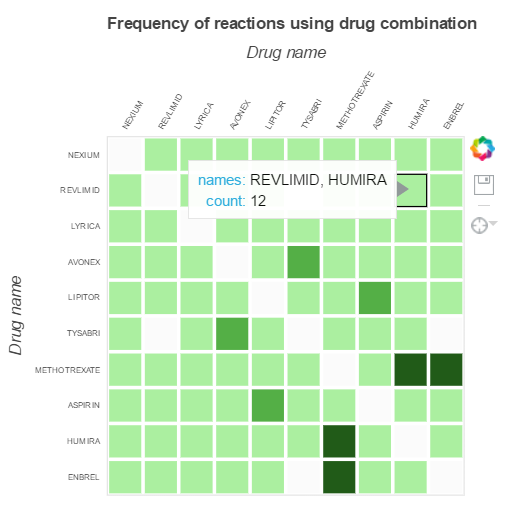
\includegraphics[width=1\textwidth]{kombinacije.png}
\end{figure}

\subsection{Najpogostejši stranski učinki}
V spodnjem grafu prikazujemo najpogostejše stranske učinke. Na abscisni osi imamo tako ponazorjeno število poročanj za neko reakcijo. Graf nam omogoča sortiranje glede na spol, čeprav je prikaz obeh spolov ves čas prikazan na grafu. To nam omogoča transparentno pregledovanje podatkov. Filtriranje je možno tudi glede na leto: izberemo lahko začetno in končno leto, torej obdobje, za katero nas zanima število poročanih stranskih učinkov. Poizvedba: \\

https://api.fda.gov/drug/event.json? \newline search=receivedate:[20040101+TO+20170106]+AND+ \newline patient.patientsex:2\& \newline count=patient.reaction.reactionmeddrapt.exact \\
\begin{figure}[H]
  \caption{Najpogostejši stranski učinki}
  \centering
    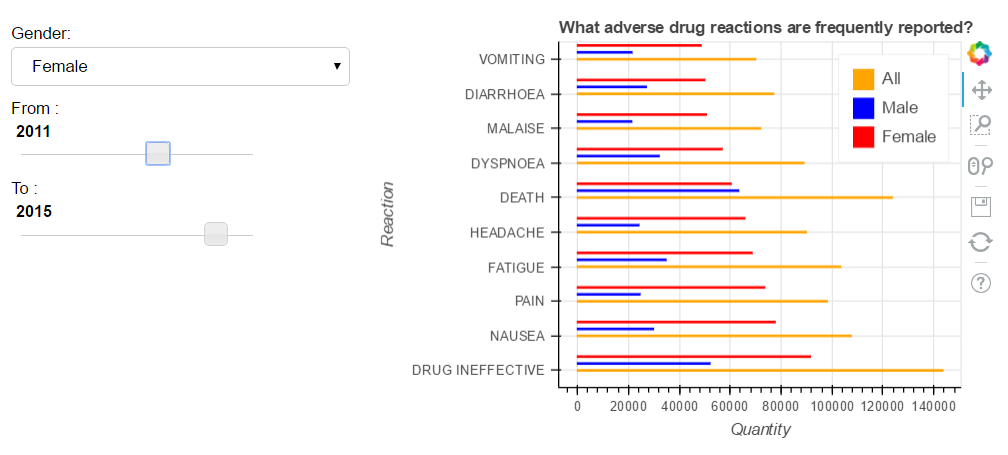
\includegraphics[width=1\textwidth]{reakcije.png}
\end{figure}

\section{Reference}
http://bokeh.pydata.org/en/latest/ \\
https://github.com/bokeh/bokeh/ \\
https://open.fda.gov/

\end{document}

